% -*- coding: utf-8 -*-
\documentclass[UKenglish,12pt]{article}
\usepackage[utf8]{inputenc}
\usepackage[T1]{fontenc,url}
%usepackage newcent for thik text
%\usepackage{babel,csquotes,textcomp}
\usepackage[top=2cm,bottom=2cm,left=2.2cm,right=2.2cm]{geometry}
%\usepackage{float}%Force figur in front of text with H - option
\usepackage{graphicx}
\usepackage{tabulary}
\usepackage{verbatim}
\usepackage{listings}
%\usepackage{bookmark} %also loads package{hyperref}
%removes: Package rerunfile check Warning: File `Essay.out' has changed.
\usepackage{bookmark}


\title{Project 2 \\ Report \\ INF4121/3121} % Title
\date{\today} % Date for the report
\author{Sebasting Søberg(INF4121) \& Thomas Oddsund(INF3121)}

% Enumerate in enumerate with numbers instead of letters
\renewcommand{\labelenumii}{\theenumii}
\renewcommand{\theenumii}{\arabic{enumii}.}


\begin{document}
\maketitle % Insert the title, author and date

\section{Requirement 1}
\subsection{Test cases}
Dynamic Technique - blacbox/experience based testing
\begin{enumerate}%all manual test cases
\item
\begin{figure}[!h]
\centering
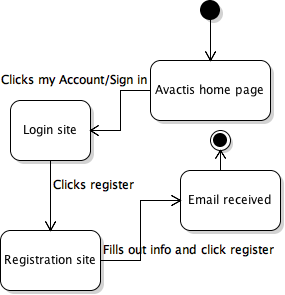
\includegraphics[scale=0.65,keepaspectratio]{Images/CreateAccount.png}
\caption{Create account state diagram}
\end{figure}
\newpage
\textbf{\hspace{0.3cm}Type\hspace{4.4cm} Description}
\newline \vspace{0.2cm}
\begin{tabular}{| p{5cm} | p{10cm} | }
	\hline
	 Title & Create account\\ \hline
	 Objective & To create a valid account that can be used for online shopping on \href{http://demo.avactis.com/4.7.9/}{\textbf{this site}.} \\ \hline
	 Pre-conditions & User have Email\\ \hline
	 Steps & \begin{enumerate} \item User opens browser \item User goes to shopping site \item User clicks \textit{My account or  Sign in} int the top right corner. \item User clicks register \item User fills in necessary information and clicks register after.\end{enumerate} \\ \hline
	 Post-conditions & \begin{enumerate} \item Website says the following in a green field: \textit{Account created successfully. You are now registered.} \item A user gets a verification email about the account registration\end{enumerate}\\ \hline
	 Expected results & User registered in avactis user database.\\ 
	 \hline
\end{tabular} % & \\ \hline

\item
%Dette diagrammet er egentlig et activity diagram, er kanskje ikke lov?
\begin{figure}[!h]
\centering
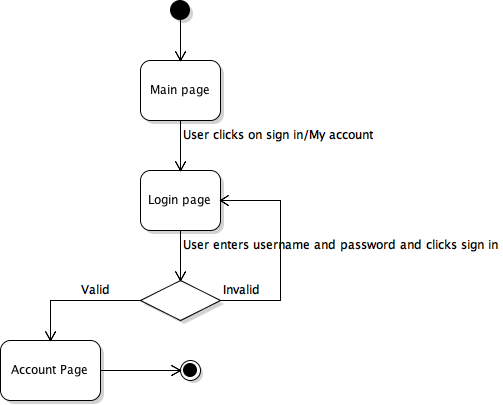
\includegraphics[scale=0.7,keepaspectratio]{Images/Login.png}
\caption{Login}
\end{figure}

\textbf{\hspace{0.3cm}Type\hspace{4.4cm} Description}
\newline \vspace{0.2cm}
\begin{tabular}{| p{5cm} | p{10cm} | }
	\hline
	 \textbf{Title} & Logging in\\ \hline
	 \textbf{Objective} & To verify that a user is registered by logging in\\ \hline
	 \textbf{Pre-conditions} & The user have a valid account\\ \hline
	 \textbf{Steps} & \begin{enumerate} \item A user opens a browser and goes to the website \item A user clicks \textit{sign in/my account} in the top right corner. \item The user fills in login details and clicks sign in \end{enumerate} \\ \hline
	 \textbf{Post-conditions} & \begin{enumerate} \item The user has an ongoing session with the shopping website \item The \textit{My Account} page loads \end{enumerate} \\ \hline
	 \textbf{Expected results} &  The user succesfully logs in and the website changes from the title \textit{sign in} in the top right corner to \textit{sign out} which indicates that you have an active session and succesfully logged in.\\ 
	 \hline
\end{tabular} % & \\ \hline


\item
\begin{figure}[!h]
\centering
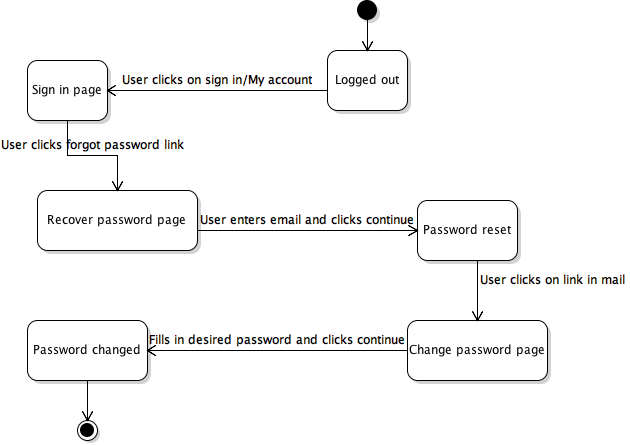
\includegraphics[scale=0.7,keepaspectratio]{Images/ResetPassword.png}
\caption{Login}
\end{figure}

\textbf{\hspace{0.3cm}Type\hspace{4.4cm} Description}
\newline \vspace{0.2cm}
\begin{tabular}{| p{5cm} | p{10cm} | }
	\hline
	 \textbf{Title} & Reset Password\\ \hline
	 \textbf{Objective} & To change or alter you password\\ \hline
	 \textbf{Pre-conditions} & A user account on avactis website\\ \hline
	 \textbf{Steps} & \begin{enumerate} \item A user opens a browser and goes to the avactis site \item The user clicks \textit{My account or Sign in} \item The under the login fields the user press the link \textit{Forgot your password?} \item The user then enters their email and click continue \item The user then clicks on the reset link in their email \item Finally the user enter their new passord \end{enumerate} \\ \hline
	 \textbf{Post-conditions} & New password to user account\\ \hline
	 \textbf{Expected results} & A user's password is updated to something new \\ 
	 \hline
\end{tabular} % & \\ \hline


\item
\begin{figure}[!h]
\centering
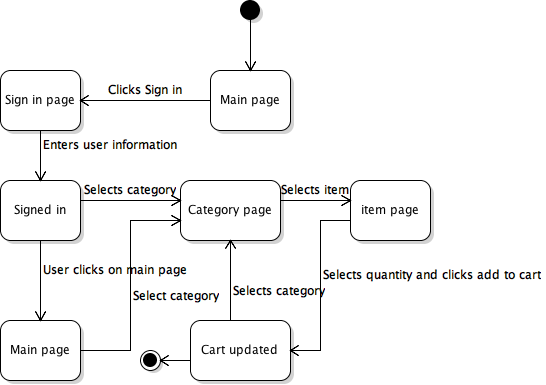
\includegraphics[scale=0.7,keepaspectratio]{Images/SelectProducts.png}
\caption{Login}
\end{figure}

\textbf{\hspace{0.3cm}Type\hspace{4.4cm} Description}
\newline \vspace{0.2cm}
\begin{tabular}{| p{5cm} | p{10cm} | }
	\hline
	 \textbf{Title} & Select Products \\ \hline
	 \textbf{Objective} & Put different products in the cart and manage the quantity of each item \\ \hline
	 \textbf{Pre-conditions} & Avactis user account \\ \hline
	 \textbf{Steps} & \begin{enumerate} \item Go to main page and click \textit{Sign in/My Account} \item Fill in username and password and click sign in \item Select categories to shop from \item Select one or more products and their quantity.
	 \end{enumerate} \\ \hline
	 \textbf{Post-conditions} & Cart contains products \\ \hline
	 \textbf{Expected results} & Cart contains products \\ 
	 \hline
\end{tabular} % & \\ \hline
%post condition vs expected results: http://www.klaros-testmanagement.com/en/forum/-/message_boards/message/144168


\item % basically this test case and diagram shall cover 3-5
\begin{figure}[!h]
\centering
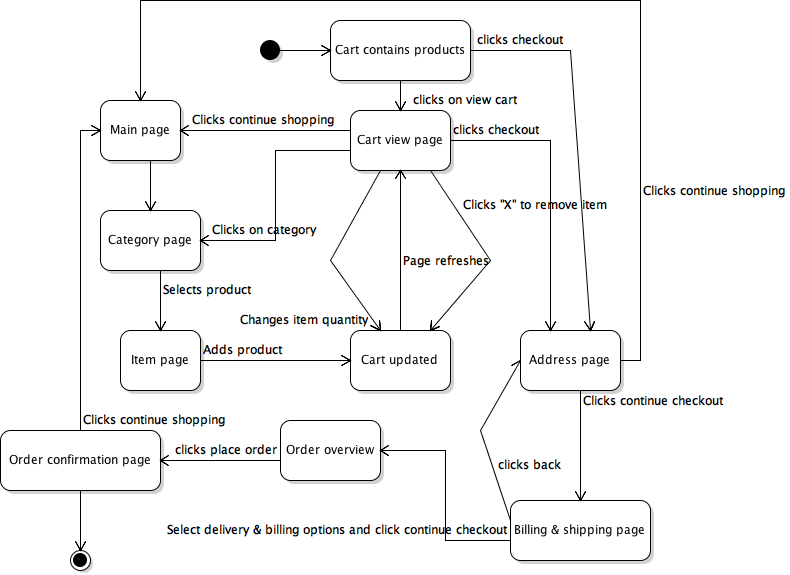
\includegraphics[scale=0.60,keepaspectratio]{Images/BuyProductsandChangeCart.png}
\caption{Shopping cart, change quantity and finalize}
\end{figure}

\textbf{\hspace{0.3cm}Type\hspace{4.4cm} Description}
\newline \vspace{0.2cm}
\begin{tabular}{| p{5cm} | p{10cm} | }
	\hline
	 \textbf{Title} & Checkout, products quantity, add/remove, finalizing and logout \\ \hline
	 \textbf{Objective} & Test that the cart indeed contains the chosen products after shopping session \\ \hline
	 \textbf{Pre-conditions} & Avactis user account and a cart of products \\ \hline
	 \textbf{Steps} & \begin{enumerate} \item Click View cart \item Change items quantity \item Click checkout \item Fill in Billing \& shipping address and click continue checkout \item Select Billing and delivery options \item Click place order
	 \end{enumerate} \\ \hline
	 \textbf{Post-conditions} & \\ \hline
	 \textbf{Expected results} & \\ 
	 \hline
\end{tabular} % & \\ \hline



\item
\begin{figure}[!h]
\centering
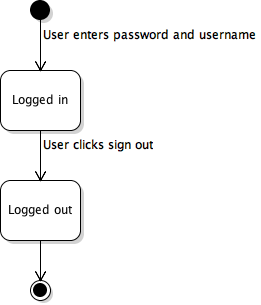
\includegraphics[scale=0.8,keepaspectratio]{Images/Logout.png}
\caption{Logout}
\end{figure}

\textbf{\hspace{0.3cm}Type\hspace{4.4cm} Description}
\newline \vspace{0.2cm}
\begin{tabular}{| p{5cm} | p{10cm} | }
	\hline
	 \textbf{Title} & Logout \\ \hline
	 \textbf{Objective} & To log out of Avactis webstore \\ \hline
	 \textbf{Pre-conditions} & A user account \\ \hline
	 \textbf{Steps} & \begin{enumerate} \item Go to Avactis homepage and click sign in \item Enter password and username \item click logout  \end{enumerate}\\ \hline
	 \textbf{Post-conditions} & \\ \hline
	 \textbf{Expected results} & \\ 
	 \hline
\end{tabular} % & \\ \hline




\item
\textbf{\hspace{0.3cm}Type\hspace{4.4cm} Description}
\newline \vspace{0.2cm}
\begin{tabular}{| p{5cm} | p{10cm} | }
	\hline
	 \textbf{Title} & \\ \hline
	 \textbf{Objective} & \\ \hline
	 \textbf{Pre-conditions} & \\ \hline
	 \textbf{Steps} & \begin{enumerate} \item 1 \end{enumerate} \\ \hline
	 \textbf{Post-conditions} & \\ \hline
	 \textbf{Expected results} & \\ 
	 \hline
\end{tabular} % & \\ \hline





\end{enumerate}

\subsection{Error on page}










\end{document}